\documentclass[crop,tikz]{standalone}
\usepackage{amsmath,amssymb,amsbsy,amsfonts,amsthm,bbm,bm,mathtools,mathrsfs}
\usepackage{tikz}
\usepackage{amsmath}
\usetikzlibrary{arrows.meta}
\usepackage{pgfplots}
\pgfplotsset{compat = newest}
\usetikzlibrary{arrows,intersections}
\usepackage{tikz-3dplot}
\usetikzlibrary{arrows,positioning} 
\tikzset{
	%Define standard arrow tip
	>=stealth',
	%Define style for boxes
	punkt/.style={
		rectangle,
		rounded corners,
		draw=black, very thick,
		text width=6.5em,
		minimum height=2em,
		text centered},
	% Define arrow style
	pil/.style={
		->,
		thick,
		shorten <=2pt,
		shorten >=2pt,}
}
\tikzset{my loop/.style =  {to path={
			\pgfextra{\let\tikztotarget=\tikztostart}
			[looseness=12,min distance=10mm]
			\tikz@to@curve@path},font=\sffamily\small
}}
\begin{document}
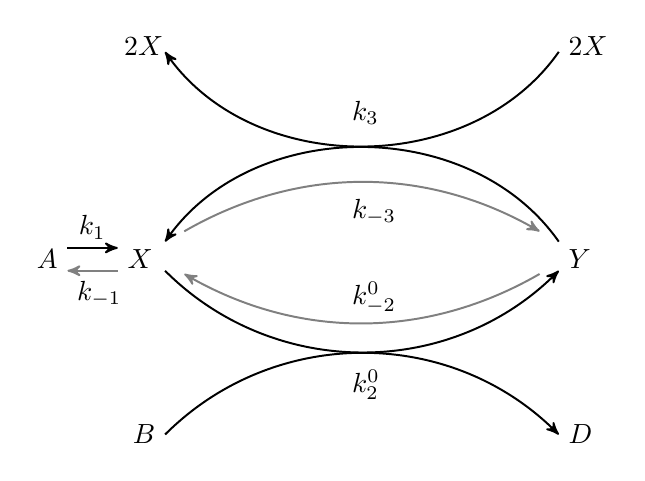
\begin{tikzpicture}[scale=1]

% first curve
 \draw[<-, line width=0.25mm, bend right=55] (0,1.43) to node[midway, above] {} (5,1.43);
 \node[left] at (0.1,1.5) {$2X$}; % 2X
 \node[right] at (5,1.5) {$2X$}; % 2X
 \node[right] at (2.25,0.66) {$k_3$}; % k3
    
  % second curve 
  \draw[<-, line width=0.25mm, bend left=55] (0,-0.98) to node[midway, above] {} (5, -0.98);

% first gray curve
\draw[->, line width=0.25mm, bend left =30, gray, shorten <=8pt, shorten >=8pt] (0, -0.99) to node[midway, below] {} (5,-0.99);
\node[right] at (2.25,-.6) {$k_{-3}$}; % k-3
  
% left straight arrow
\node[right] at (-0.60,-1.2) {$X$}; % X (right)
 \draw[->, line width=0.25mm] (-1.24, -1.06) -- node[midway, above] {} (-0.6, -1.06);  
  \draw[<-, line width=0.25mm, gray] ((-1.24,-1.35) -- node[midway, above] {} (-0.6,- 1.35);  % gray 
\node[left] at (-1.24,-1.2) {$A$}; % A (left)

\node[right] at (-1.22,-0.8) {$k_1$}; %k1
\node[right] at (-1.24,-1.65) {$k_{-1}$}; %k1

\node[right] at (5,.-1.2) {$Y$};


% second gray curve
  \node[right] at (2.25,-1.7) {$k^0_{-2}$}; % k_0 -2 
\draw[<-, line width=0.25mm, bend right =30, gray, shorten <=8pt, shorten >=8pt] (0, -1.25) to node[midway, below] {} (5,-1.25);

% third curve
  \draw[->, line width=0.25mm, bend right=45] (0,.-1.35) to node[midway, above] {} (5,-1.35);
  
  % fourth curve
  \draw[->, line width=0.25mm, bend left=45] (0,-3.43) to node[midway, above] {} (5, -3.43);
    \node[left] at (0.,-3.43) {$B$}; % B
  \node[right] at (5,-3.43) {$D$}; % D
  \node[right] at (2.25,-2.8) {$k_2^0$}; % k_2 0
    
 \end{tikzpicture}

\end{document}

